\documentclass{article}
\usepackage[T1]{fontenc}
\usepackage{times}
\usepackage{geometry}
\geometry{a4paper,left=0.6cm,right=0.7cm,top=1.5cm,bottom=1cm,columnsep=0.8cm}
\usepackage[utf8]{inputenc}
\usepackage{textcomp}
\usepackage{newtxtext}
\usepackage{fontawesome}          % icônes de base seulement
\usepackage[hidelinks]{hyperref}
\usepackage{multicol}
\usepackage{tikz}
\usepackage{hyphsubst}
\usepackage{moresize}
\usepackage{hyphenat}
\usepackage{tabularx}
\usepackage{ragged2e}
\usepackage{xcolor}
\usepackage{enumitem}
\usetikzlibrary{calc, positioning}
\newcolumntype{Y}{>{\RaggedRight\arraybackslash}X}

% icônes manquantes -> puce
\makeatletter
\@for\sym:=faBrain,faMicrochip,faHandshakeO,faTools,faNetworkWired,%
             faDatabase,faServer,faGit,faUsers,faComments,faCalendar,faGroup\do{%
  \@ifundefined{\sym}{\expandafter\newcommand\csname\sym\endcsname{\textbullet}}{}}
\makeatother

% couleurs
\definecolor{maincolor}{HTML}{f0fafc}
\definecolor{seccolor}{HTML}{ffffff}
\definecolor{gray}{HTML}{8c94a9}
\definecolor{sidetext}{HTML}{59cee5}

% bande latérale bleue
\usepackage{eso-pic}
\AddToShipoutPictureBG{%
  \begin{tikzpicture}[remember picture,overlay]
    \fill[maincolor] (current page.north west) rectangle
                     ([xshift=0.3\paperwidth] current page.south west);
  \end{tikzpicture}%
}

% listes
\setlist[itemize]{itemsep=-2pt,topsep=0pt,leftmargin=1.08cm}
\renewcommand{\labelitemi}{\textcolor{sidetext}{\footnotesize$\bullet$}}

\setlength{\parindent}{0pt}
\usepackage{paracol}
\columnratio{0.3}

\begin{document}
\pagestyle{empty}

\begin{paracol}{2}
% ────────────────────────────────────────
% Colonne gauche
% ────────────────────────────────────────
\color{sidetext}
\vspace*{-0.5cm}


\noindent
\begin{minipage}{\linewidth}
  \centering
  \ifx\relaxd636a17c9cf6472988ce2da23437bf5d.jpg\relax\else
  \begin{tikzpicture}
    \clip (0,0) circle (1.5cm) node[anchor=center]
      {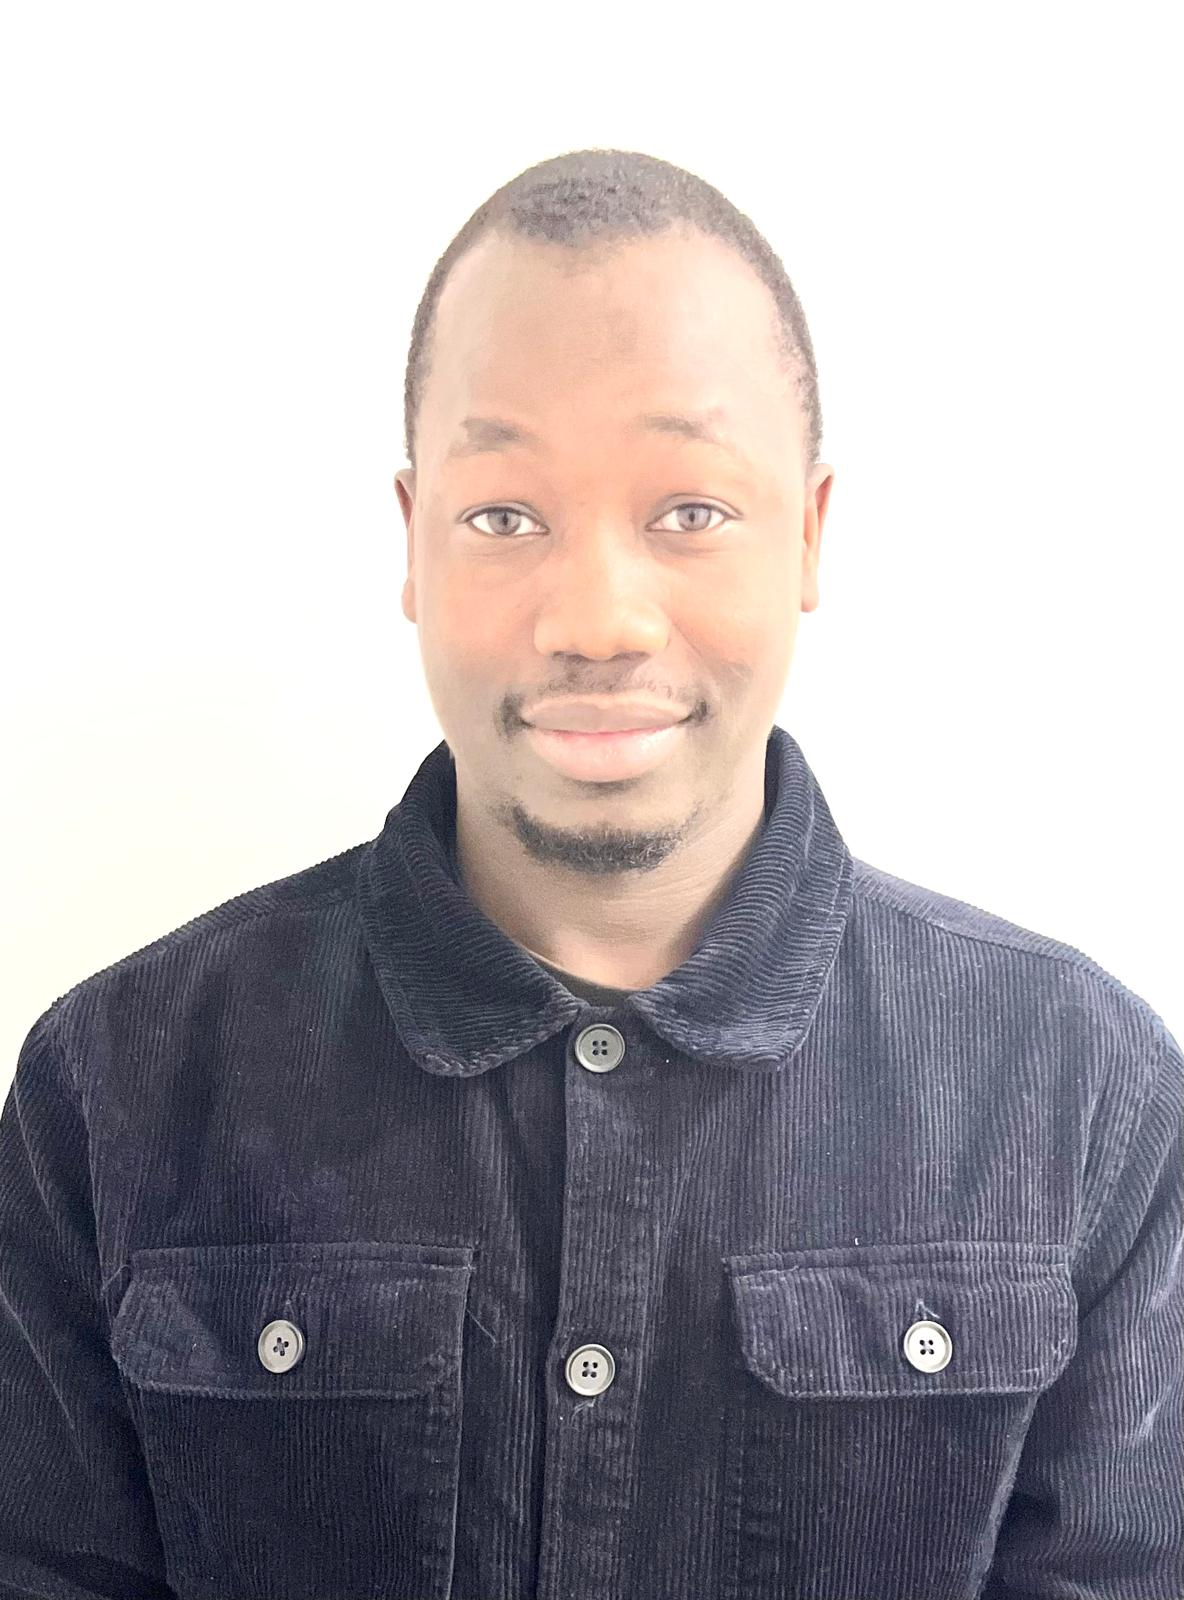
\includegraphics[width=3cm]{d636a17c9cf6472988ce2da23437bf5d.jpg}};
  \end{tikzpicture}
  \fi

  \vspace{3mm}
  {\color{black}\LARGE \textbf{Pape Saliou FALL}}

  \vspace{1mm}
  {\large Ingénieur Data Scientist et Développeur IA}

  \vspace{3mm}
  {\color{gray}\rule{\linewidth}{0.4pt}} \\
\end{minipage}

% ── Coordonnées
\begin{tabular}{@{}c l}
  \faPhone &
  \begin{tabular}[t]{@{}l@{}}
    {\color{gray}Téléphone} \\ 0753481453
  \end{tabular} \\
  \\
  \faLinkedin &
  \begin{tabular}[t]{@{}l@{}}
    {\color{gray}LinkedIn} \\
    \href{@pape-saliou-fall-43154a211/}{}
  \end{tabular} \\
  \\
  \faMapMarker &
  \begin{tabular}[t]{@{}l@{}}
    {\color{gray}Adresse} \\ 95300 Pontoise \\ 
  \end{tabular} \\
  \\
  \faEnvelope &
  \begin{tabular}[t]{@{}l@{}}
    {\color{gray}Email} \\
    \href{mailto:papesalioufall2@gmail.com}{papesalioufall2@gmail.com}
  \end{tabular} \\
\end{tabular}

\vspace{2mm}
{\color{gray}\rule{\linewidth}{0.4pt}} \\

% ── Langues --------------------------------------------------------
{\color{black}{Langues}}

\vspace{2mm}
\begin{itemize}[leftmargin=*]
\item Français - \textcolor{gray}{Natif}
\item Anglais - \textcolor{gray}{B2}\end{itemize}          % ← le placeholder va contenir \begin{itemize}…\end{itemize}
\vspace{2mm}
{\color{gray}\rule{\linewidth}{0.4pt}} \\

% ── Compétences ----------------------------------------------------
\vspace{2mm}
{\color{black}{Compétences Clés}}

\vspace{2mm}
\begin{itemize}[leftmargin=*]
\item Python
\item SQL
\item Tensorflow
\item Scikit-learn
\item PowerBI
\item Git
\item Flask\end{itemize}              % ← idem, une vraie liste
\vspace{2mm}
{\color{gray}\rule{\linewidth}{0.4pt}} \\

% ── Centres d'intérêt
\vspace{2mm}
{\color{black}{Centres d’intérêt}}

\vspace{2mm}
\begin{itemize}[leftmargin=*]
\item Football
\item Natation
\item Lecture
\end{itemize}     % ← simple itemize ou tabular

\vfill
~

% ────────────────────────────────────────
\switchcolumn
% Colonne droite
% ────────────────────────────────────────
\color{black}

% ── Profil
\textcolor{black}{\Large \textbf{Profil Professionnel}} \\[2pt]
Ingénieur statisticien et data scientist de formation, j’assure aujourd’hui la conception complète de plateformes web exploitant des modèles d’IA générative (GPT-4o, GPT-3.5-turbo, Gemini). Du back-end Python/Flask à l’interface front-end HTML/CSS/JavaScript, je prends en charge tout le cycle de développement jusqu’au déploiement continu (Git, Heroku). J’automatise également les workflows métiers avec Zapier afin d’accélérer la mise en production et de maximiser la valeur ajoutée produit. Autonome, rigoureux et passionné par l’innovation, je souhaite mettre mon double profil data \& développement au service d’une équipe ambitieuse. \\[8pt]

% ── Expérience
\textcolor{black}{\Large \textbf{Expérience Professionnelle}} \\[2pt]
\colorbox{maincolor}{%
  \begin{minipage}{\linewidth}
    \noindent
    \textbf{Data Scientist \& Développeur IA}\hfill depuis 01/2024\\
    Prepaya\\[-0.3em]
    \begin{itemize}[leftmargin=*]
      \item Développé de bout en bout (backend Python/Flask \& frontend HTML/CSS/JavaScript) plusieurs plateformes SaaS intégrant des modèles LLM (GPT-4o, GPT-3.5-turbo, Gemini) et totalisant plus de 1 000 utilisateurs actifs. \item Industrialisé les workflows IA : fine-tuning des modèles, packaging Docker, déploiement automatisé sur Heroku via Git et pipelines CI/CD. \item Implémenté des automatisations métier (Zapier) et des API REST sécurisées, réduisant de 40 \% le temps de traitement client.
    \end{itemize}
  \end{minipage}}

\vspace{3mm}

\colorbox{maincolor}{%
  \begin{minipage}{\linewidth}
    \noindent
    \textbf{Apprenti Risk Analyst \& Data Scientist}\hfill 12/2022 - 12/2023\\
    AXA XL (Groupe AXA)\\[-0.3em]
    \begin{itemize}[leftmargin=*]
      \item Automatisé la collecte de données financières (Python, VBA, SQL), supprimant les tâches manuelles répétitives. \item Construit des tableaux de bord Power BI pour le suivi de la facturation et le reporting à la direction financière. \item Mis au point des modèles prédictifs permettant d’estimer la probabilité de sinistre par client.
    \end{itemize}
  \end{minipage}}

\vspace{3mm}

\colorbox{maincolor}{%
  \begin{minipage}{\linewidth}
    \noindent
    \textbf{Apprenti Data Scientist}\hfill 09/2021 - 08/2022\\
    Prepaya\\[-0.3em]
    \begin{itemize}[leftmargin=*]
      \item Déployé des modèles NLP (BERT, T5) afin de générer automatiquement des formulaires structurés. \item Réalisé une analyse de sentiment des retours clients pour identifier les axes d’amélioration. \item Industrialisé la collecte et le pré-traitement de données web (BeautifulSoup, Selenium).
    \end{itemize}
  \end{minipage}}   % ← blocs \colorbox{maincolor}{\begin{minipage}…}

\vspace{8mm}

% ── Formation
\textcolor{black}{\Large \textbf{Formation}} \\[2pt]
\colorbox{maincolor}{%
  \begin{minipage}{\linewidth}
    \noindent
    \textbf{Master 2 Data Science}\hfill 09/2021 - 03/2022\\
    Sorbonne Université\\[-0.3em]
    \begin{itemize}[leftmargin=*]
      \item Machine learning avancé, deep learning et séries chronologiques. \item Statistiques, bases de données et data visualisation. \item Programmation Python/R et calcul parallèle.
    \end{itemize}
  \end{minipage}}       % ← lignes tabular par diplôme

\end{paracol}
\end{document}

